\documentclass[11pt, a4paper]{article}
\usepackage[utf8]{inputenc}
\usepackage[T1]{fontenc}
\usepackage[top=2.5cm, bottom=2.5cm, left=1.5cm, right=2cm]{geometry}
\usepackage{graphicx}
\usepackage{xcolor}

\newcommand{\addressed}{We thank the reviewer for the comment, which has been addressed in the manuscript. Changes were done accordingly.}

\newcommand{\response}[1]{\textcolor{blue!50!black}{- #1}}

\begin{document}
\begin{center}
    \begin{Large}
        \textbf{Response Letter to Reviewers}\\[1em]
    \end{Large}
    Article reference: JAP24-AR-05791R \\ A general spectral collocation method for computing the dispersion relations of guided acoustic waves in multilayer dissipative structures
\end{center}

\vspace*{1cm}

We thank again the associate editor for their interest in our paper and to the reviewers for their feedback. We are grateful for the proposition for publication formulated by Reviewer 2. In this response letter, we focus on the last comment from Reviewer 3 regarding the comparison to SAFE that was requested. We remind the reviewer of our last answer to this suggestion which was:

\emph{"- It would have indeed been interesting to compare our SCM with some SAFE simulations, although this work does not provide an extensive review of the existing numerical methods to compute
dispersion curves. Nevertheless, we do not agree with the  tatement that SAFE is the most accurate method for this kind of computation. There is already a large literature, including some books cited in our paper that discuss the fundamental aspects of SAFE and SCM, as well as the reference by A. Huber [2] that you provided in your next comment. The SCM is known as similar to SAFE due to the discretization in one dimension and a semi-analytical wave propagation in the other dimension that they both use. The key differences appear in the much faster computation time and higher accuracy achieved by the SCM. This is a point we were aware of from the outset of our work, in
order to identify the most appropriate method for us"}. 

We still stand by this opinion about our work and still think that comparing these two methods is out of scope for our paper. However, we provide some additional insight on the subject in the following of the letter.

\begin{figure}[h!]
    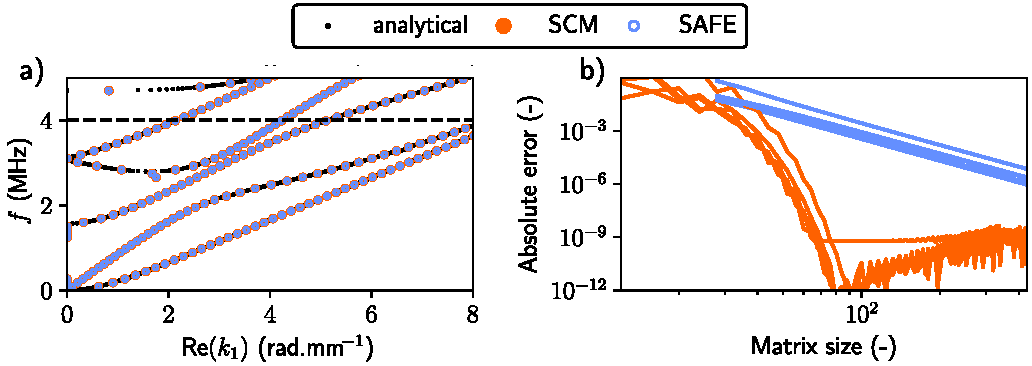
\includegraphics{figure.pdf}
    \caption{a) Dispersion relation of the Lamb modes: root-finding analytical method (black), SCM (orange) and SAFE (blue). The dashed line shows the selected frequency for the convergence study. b) Convergence of the 2 methods at a given frequency $f=$ 4 kHz shown in log-log scale. Each line corresponds to a specific wavenumber and is color-matched with the method used.}
    \label{fig:figure}
\end{figure}

The specific situations that we chose for a comparison between our current method (SCM) and SAFE is that of Lamb modes, which is a classical configuration for dispersion curve calculation. A layer of elastic material (aluminium in our case) of infinite extent along the longitudinal direction, has a thickness $L = 1$mm. We derive the SAFE method for this case, following the approach proposed in Chapter 9 of Joseph Rose's book \footnote{J. L. Rose, \textit{Ultrasonic Guided Waves in Solid Media}, Cambdridge (2014)}. The interpolating shape functions used are the same as those used in the previous reference, that is second-order Lagrange polynomials. We do not recall the derivation steps for sake of conciseness.

The results from our analysis are provided in Fig.~\ref{fig:figure}. Therein, we compare the dispersion curves given by the two numerical methods. For validation, we also provide the analytical dispersion curve of Lamb modes, obtained by solving the Lamb dispersion equations\footnote{D. Royer and T. Valier-Brasier, \textit{Ondes élastiques dans les solides}, ISTE Éditions (2021)} using our root-finding method, which was described in our paper. Figure~\ref{fig:figure}a) depicts the dispersion curve for real wavenumbers computed using the three methods: analytical results from root-finding, SCM and SAFE. It can be seen that the same dispersion curve is retrieved in each case, thus validating our SAFE implementation.

The convergence curves are depicted in Fig.~\ref{fig:figure}b). There, the absolute error between each numerical method with respect to the analytical solution is computed at a given frequency chosen as 4 MHz. The matrix size $n$ is chosen as the way to compare the two methods discretizations, computed by sweeping the number of elements from $m=3$ to $m=60$. The SCM matrix size is $n = 2m$ while for SAFE, it is $n = 2(2m + 1)$. For each method, the eigenvalue problem is written by augmenting the problem size by a factor 2. The results obtained from the convergence are unsurprisingly in agreement with the literature. The SCM convergence shows an exponential decrease and reaches a dip in error around $m = 20$ (matrix size around $n=80$), while the SAFE curve follows a slope of order 3 which is expected from a finite elements method that uses second-order shape functions. 

From this analysis, we assert that SCM performs much better than our implementation of SAFE. These results are not new and are backed by several evidences in the literature, as discussed earlier in the letter and in the paper. The authors want to stress that the comparison between our method and SAFE is out of the scope of the current paper, although we thank again the reviewer for opening such discussion.

\end{document}